\section{CIE 2006-XYZ空间}
题目中第三个任务为使用CIE 2006-XYZ色彩空间的色彩匹配函数(三刺激值)替换掉CIE 1931-XYZ的色彩匹配函数。重新画出色品图以及比较。画色品图的流程基本与上一节一样,对CIE 2006-XYZ 380$\sim$389nm的xyz值缺失采用0填充。

\subsection{CIE 2006-XYZ空间 -- 色品图}

CIE 2006-XYZ空间的色品图绘制与CIE 1931-XYZ空间上的绘制完全一致,只是三刺激值有所改变。如图\ref{fig:tri-xyz}与\ref{fig:tri-xyz-2}所示,色彩匹配函数大同小异,其结果估计也相近。2006与1931的色彩匹配函数得到的马蹄图轮廓区别如图\ref{fig:cmp-sd}所示。

\begin{figure}[htbp]
    \centering
    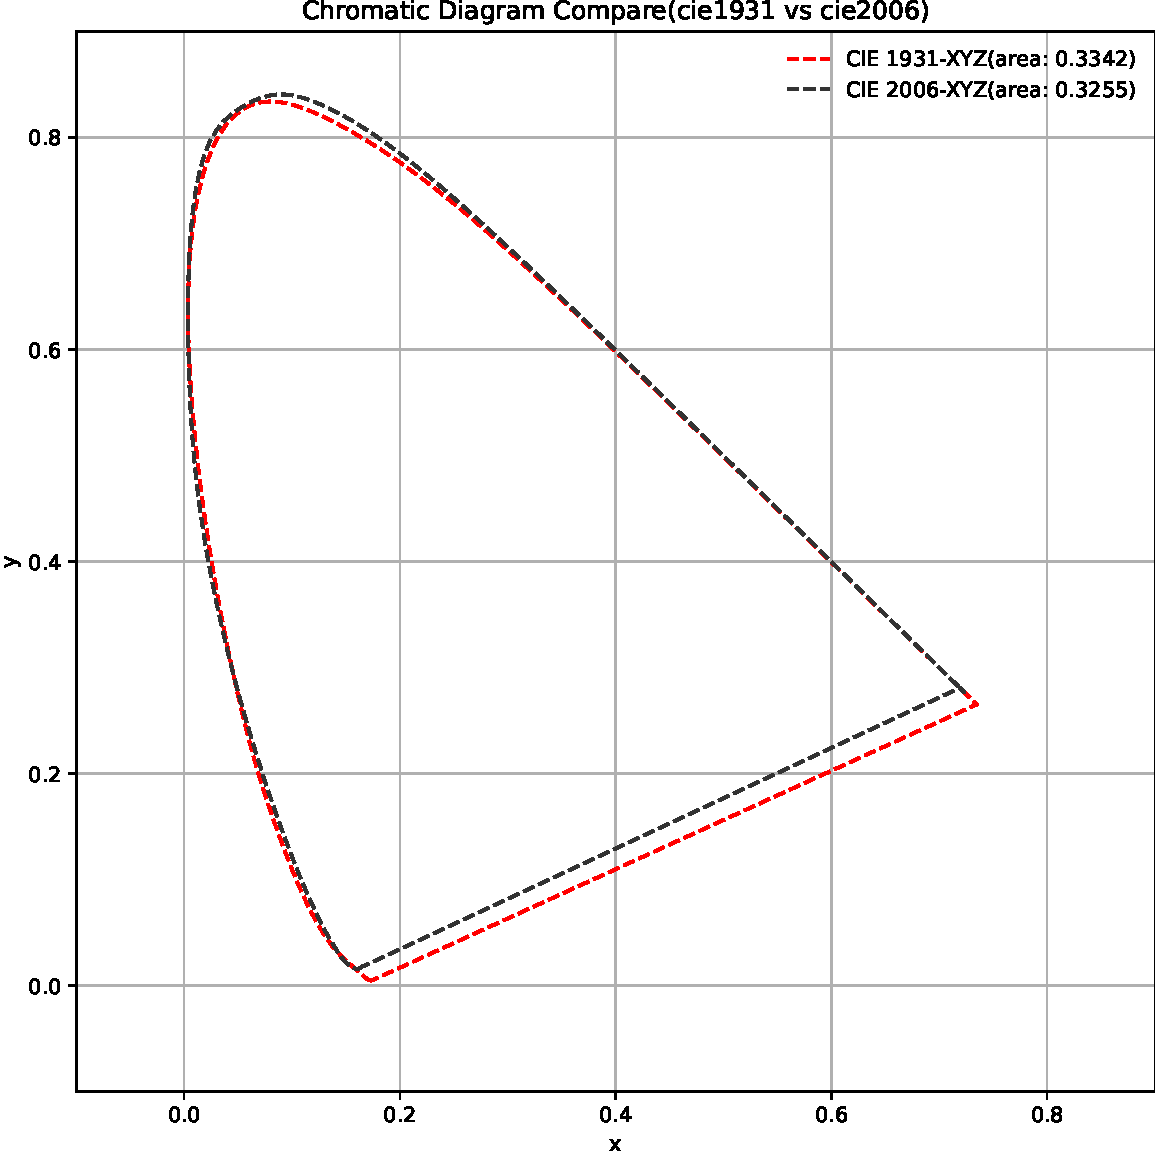
\includegraphics[width=0.65\textwidth]{./imgs/sec4/cmp-sd.pdf}
    \caption{两种色彩匹配函数的轮廓比较图}
    \label{fig:cmp-sd}
\end{figure}

从图中我们可以知道CIE 2006的马蹄图的面积为0.3255,比CIE 1931的马蹄图,主要差异在于左下角填0处(间接导致直线偏离),从三刺激值图中我们也可以看出蓝色光更集中了,蓝色``缺了一块'',绿色区域稍有变动,总体改变不大,由于我们使用的转sRGB的公式并没有发生变化,因此底色背景是没有区别的。

\subsection{绘制CIE 2006-XYZ空间色域}

\begin{figure}[htbp]
    \centering
    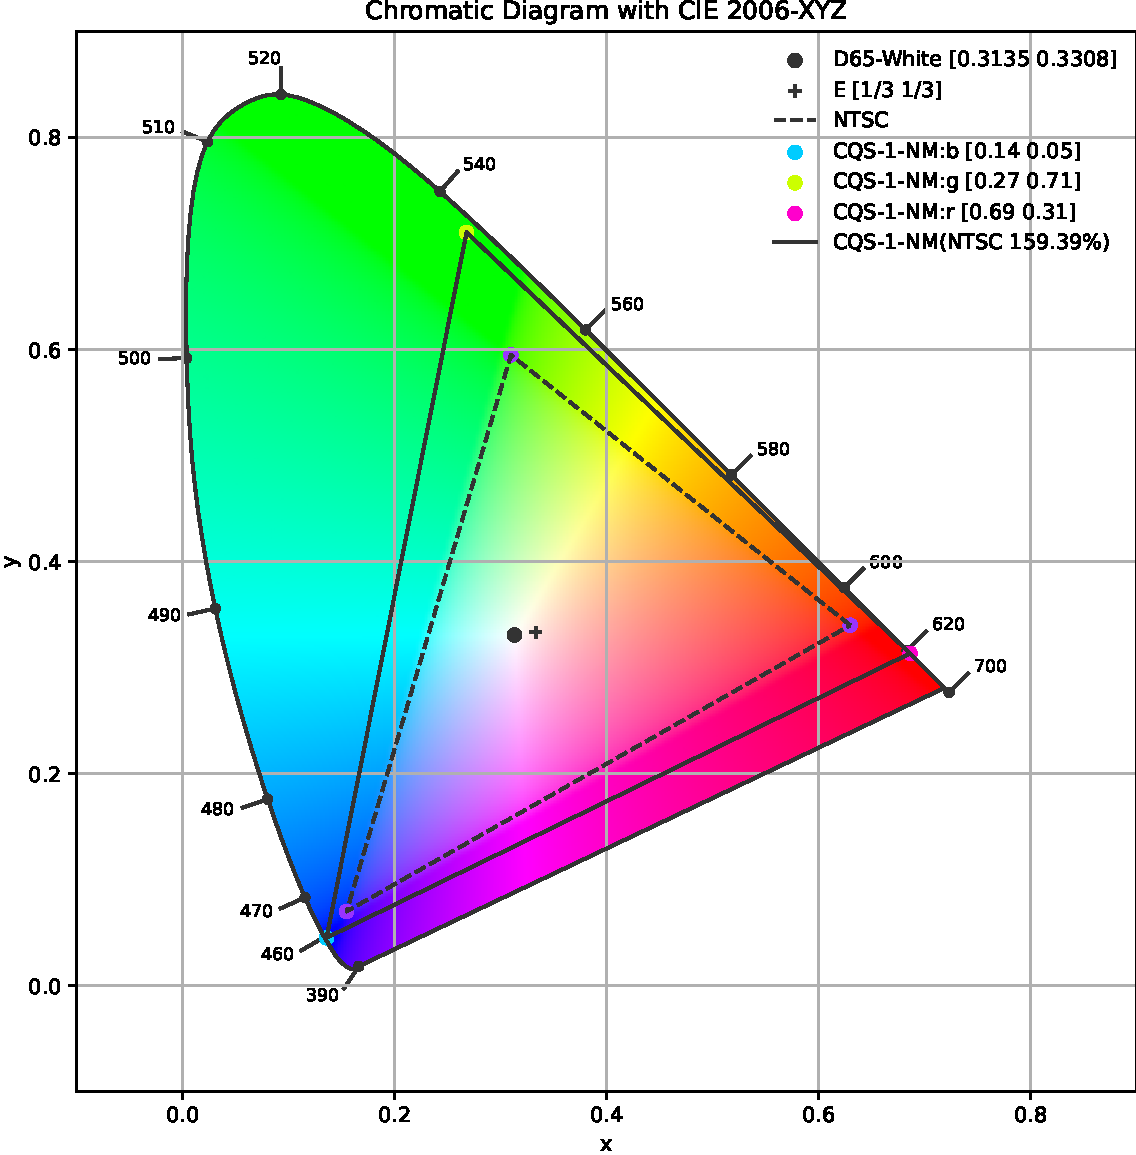
\includegraphics[width=0.65\textwidth]{./imgs/sec4/CQS-1-NM-2006-sd.pdf}
    \caption{CIE 2006-XYZ色彩匹配函数下的LED色域与NTSC色域}
    \label{fig:sd2006-ledwithntsc}
\end{figure}

\begin{figure}[htbp]
    \centering
    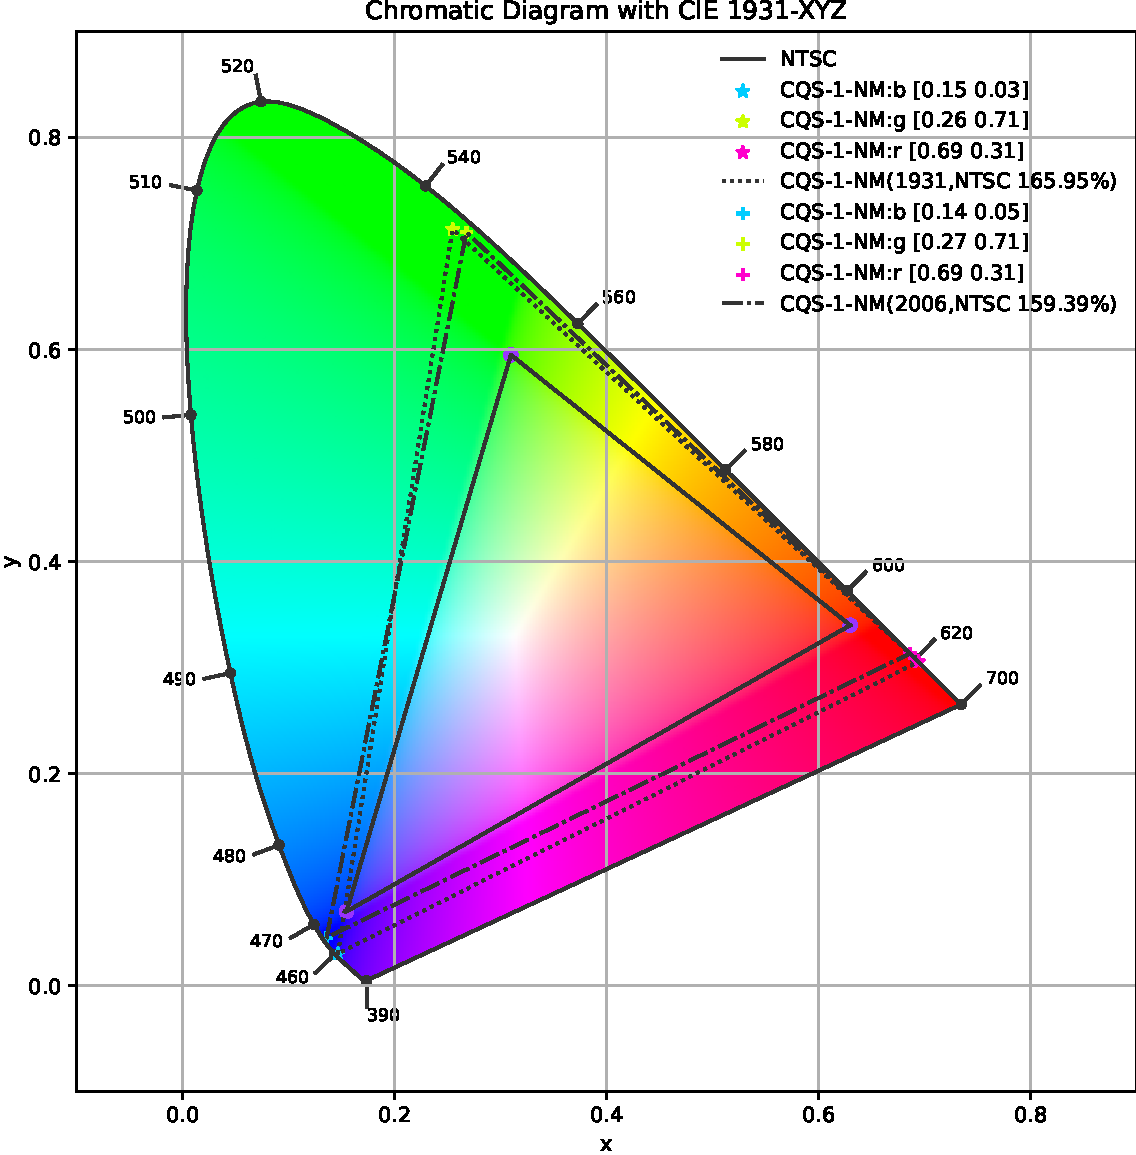
\includegraphics[width=0.65\textwidth]{./imgs/sec4/CQS-1-NM-cmparea-sd.pdf}
    \caption{CIE 1931-XYZ与CIE 2006-XYZ色彩匹配函数下的色域对比}
    \label{fig:sd1931vs2006}
\end{figure}

与图\ref{fig:sd1931-ledwithntsc}绘制步骤相同我们可以获得CIE 2006-XYZ空间的色品图与色域,结果如图\ref{fig:sd2006-ledwithntsc}所示,乍得一看与CIE 2006-XYZ区别不大,相比于CIE 1931-XYZ而言仅仅是蓝光和绿光的坐标点在横坐标中移动了$0.1$,色域范围发生了相对较大的变化,从``NTSC 165.95\%''转变为``NTSC 159.39\%'',但我感觉主要的原因是NTSC制定的时候是通过CIE 1931-XYZ的色彩匹配函数确定的,而我们并没有NTSC的红绿蓝三色的标准光谱,这个NTSC色域的数据点没有重新计算而是直接迁移到CIE 2006-XYZ,因此造成了色域定量表示的误差。我觉得并没有太大的区别。接下来我按照第三个子目标的前半要求将这两个结果绘制在同一张图上,并以CIE 1931-XYZ的色品图作为背景(也可以绘制在CIE 2006-XYZ),结果如图\ref{fig:sd1931vs2006}所示。

\subsection{多种对比}

我从欧司朗OSRAM\footnote{https://www.osram.com/apps/downloadcenter/os/?path=\%2Fos-files\%2FOptical+Simulation\%2FLED\%2F}也找到了RGB三色光的灯泡数据,但是由于水平与时间的双不足,我不太清楚它和llab是否是同一种光源技术,在此我们假设它们是不同的光源技术(因为数据太难找了,我只找到这几个能用的)。

首先我们选择OSCONIQ的两个系列的彩色LED灯,型号分别为P2226\footnote{https://www.osram.com/apps/downloadcenter/os/?path=\%2Fos-files\%2FOptical+Simulation\%2FLED\%2FOSCONIQ\\\%2FOSCONIQ+P\%2FOSCONIQ+P2226\%2F}与P3030\footnote{https://www.osram.com/apps/downloadcenter/os/?path=\%2Fos-files\%2FOptical+Simulation\%2FLED\%2FOSCONIQ\\\%2FOSCONIQ+P\%2FOSCONIQ+P3030\%2F}系列。

P2226选用了GD\_DASPA2作为蓝色灯、GR\_DASPA2作为红色灯、GT\_DASPA2作为绿色灯。相对光谱分布(通道归一化)如图\ref{fig:P2226}所示。

\begin{figure}[htbp]
    \centering
    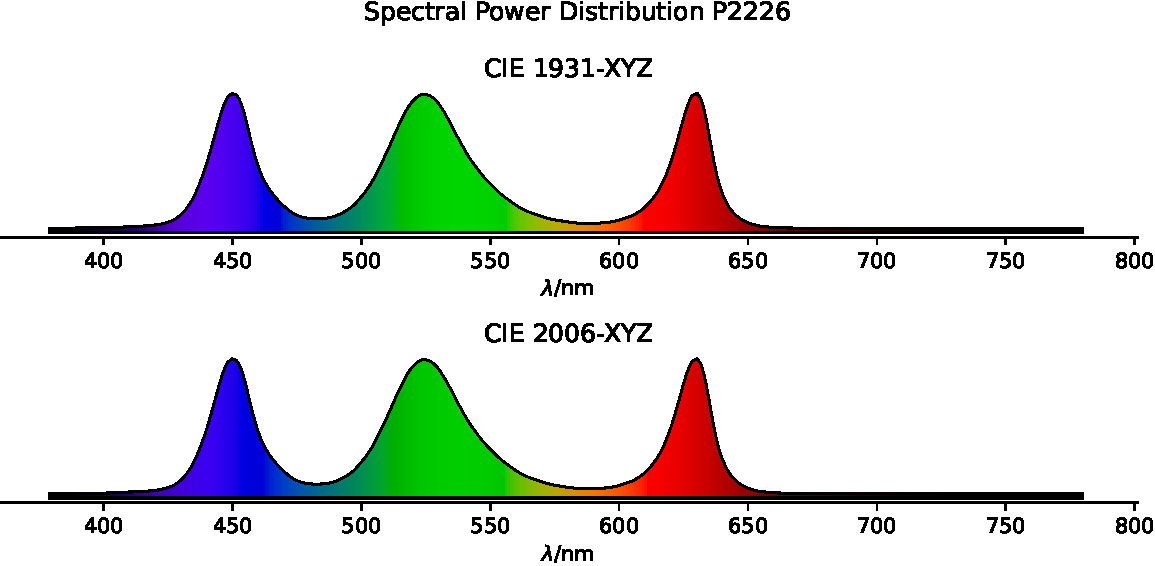
\includegraphics[width=0.65\textwidth]{./imgs/sec4/P2226-spd-n.pdf}
    \caption{P2226相对光谱分布图}
    \label{fig:P2226}
\end{figure}

P3030选用了GD\_DASPA2作为蓝色灯、GR\_DASPA2作为红色灯、GT\_DASPA2作为绿色灯。相对光谱分布(通道归一化)如图\ref{fig:P3030}所示。

\begin{figure}[htbp]
    \centering
    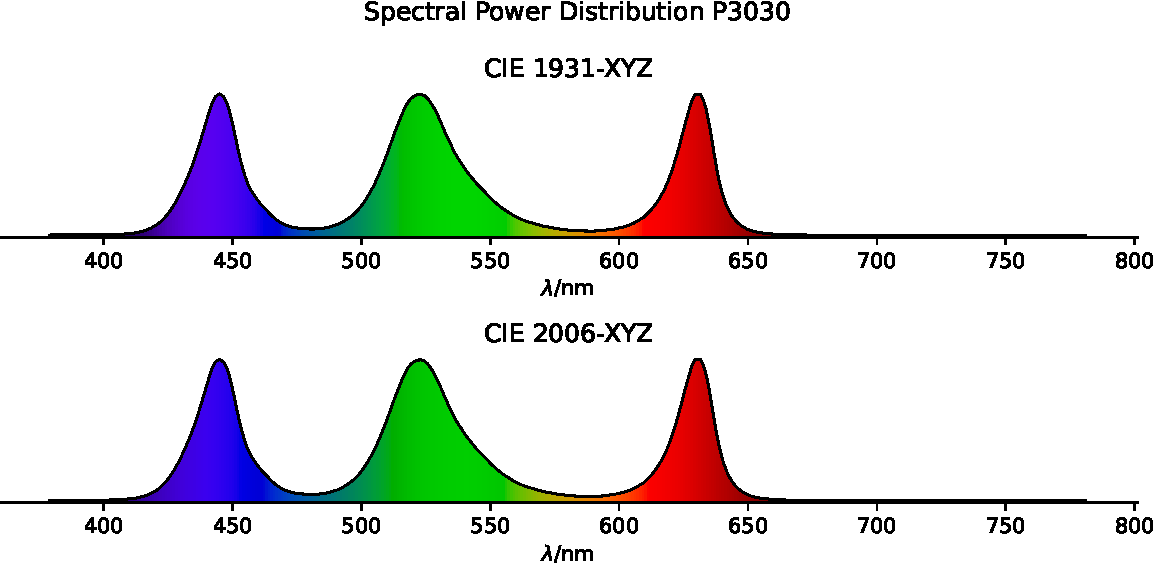
\includegraphics[width=0.65\textwidth]{./imgs/sec4/P3030-spd-n.pdf}
    \caption{P3030相对光谱分布图}
    \label{fig:P3030}
\end{figure}

由于P2226和P3030数据是以2nm为间隔的,为了方便统一处理,本文使用了三次样条插值进行处理,对部分光谱非固定间隔的进行了固定间隔化。结果如图\ref{fig:cmpdifled}所示。

\begin{figure}[htbp]
    \centering
    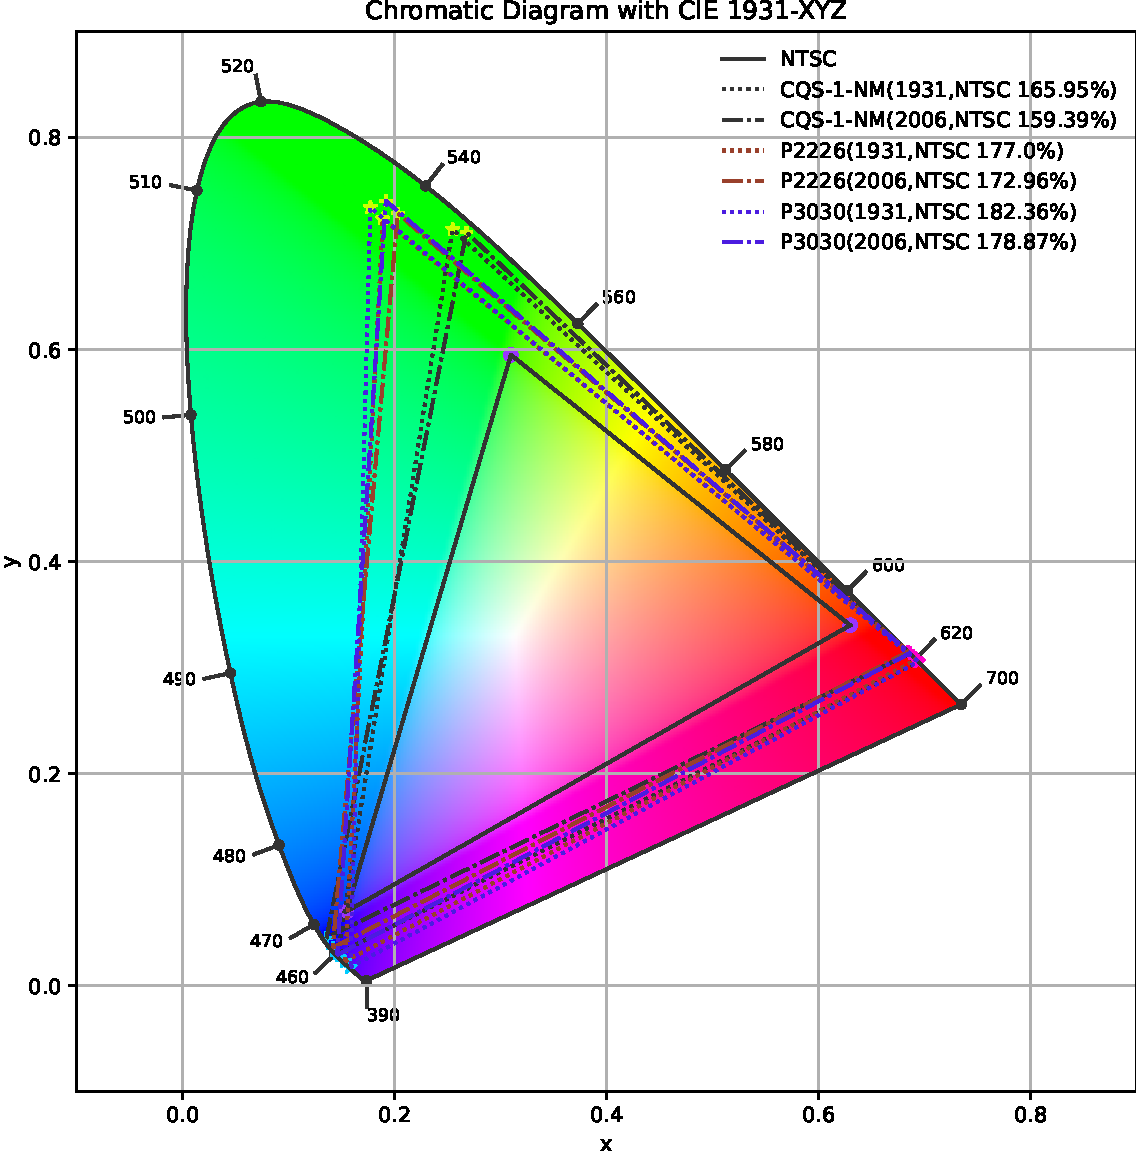
\includegraphics[width=0.65\textwidth]{./imgs/sec4/P3030-cmparea-sd.pdf}
    \caption{三种LED在两种色彩匹配函数中的色域对比}
    \label{fig:cmpdifled}
\end{figure}

从图中我们可以得知,两种色彩匹配函数表现的效果基本类似,圈定的范围重合度很高。从图上我们可以得到一个结论,3种LED的色域绿色都会向着左下角偏移(深绿),蓝色都会向着深蓝偏移(右下),红色基本不变,这是因为在2006版的色彩匹配函数中蓝色$\overline z$更集中了,导致蓝绿色在积分的时候Z值会更大,从而影响坐标,对R光而言较为远离影响不大。

从图中我们同时可以知道从1931转到2006,llab和P3030的LED的色域都减小了一点,P2226LED的色域反而增大了。我们观摩三个LED的相对光谱图\ref{fig:spd1931bgn},\ref{fig:P2226},\ref{fig:P3030}可以知道,llab和P3030相对于P2226来说更远离2006-XYZ的蓝色峰值,导致组成色域的蓝色点更接近其他两点,导致面积变小,色域定量范围变小,而P2226是更接近2006-XYZ蓝色峰值,因此色域变大,但影响都不大。总得来说这两种色彩匹配函数在实际应用中并没有很大的区别,只是蓝光处有些许影响。